\documentclass[fleqn]{article}
\usepackage[nodisplayskipstretch]{setspace}
\usepackage{amsmath, nccmath, bm}
\usepackage{amssymb}
\usepackage{enumitem}
\usepackage{etoolbox}
\usepackage{graphicx}
\usepackage{float}
\usepackage{changepage}
\usepackage{environ,capt-of}

\let\oldfigure\figure% Store original figure float environment
\let\endoldfigure\endfigure
\RenewEnviron{figure}[1][H]{% Update figure environment
  %\par\vspace{\intextsep}% Assume in-text placement, so insert appropriate vertical spacing
  \noindent
  % \patchcmd{<cmd>}{<search>}{<replace>}{<success>}{<failure>}
  \patchcmd{\BODY}{\caption}{\captionof{figure}}{}{}% Replace \caption with \captionof{figure} inside \BODY
  % Set "figure"
  \begin{minipage}{\linewidth}
    \BODY
  \end{minipage}
  %\par\vspace{\intextsep}% Assume in-text placement, so insert appropriate vertical spacing
}

\newcommand{\zerodisplayskip}{
	\setlength{\abovedisplayskip}{0pt}%
	\setlength{\belowdisplayskip}{0pt}%
	\setlength{\abovedisplayshortskip}{0pt}%
	\setlength{\belowdisplayshortskip}{0pt}%
	\setlength{\mathindent}{0pt}}
	
\newcommand{\norm}[1]{\left \lVert #1 \right \rVert}

\makeatletter
\renewcommand*\env@matrix[1][*\c@MaxMatrixCols c]{%
	\hskip -\arraycolsep
	\let\@ifnextchar\new@ifnextchar
	\array{#1}}
\makeatother

\title{Homework 3}
\author{Owen Sowatzke}
\date{March 13, 2024}

\begin{document}

	\offinterlineskip
	\setlength{\lineskip}{12pt}
	\zerodisplayskip
	\maketitle
	
	\begin{enumerate}
		\item The exclusive-OR is the simplest problem that cannot be solved using a linear discriminant operating directly on the features. The points $k=1,3$ at $\mathbf{x} = [1,1]^T$ and $[-1,-1]^T$ are in the category $\omega_1$ (red in the figure), while $k=2,4$ at $\mathbf{x}=[1,-1]^T$ and $[-1,1]^T$ are in $\omega_2$ (black in the figure). Following the approach of Support Vector Machines, we preprocess the features to map them to a higher dimension space where they can be linearly separated. While many $\varphi$-functions could be used, here we use the simplest expansion up to second order: $1, \sqrt{2}x_1, \sqrt{2}x_2, \sqrt{2}x_1x_2, x_1^2$ and $x_2^2$, where the $\sqrt{2}$ is convenient for normalization. Using the support vector machine formulation, show that the optimum discriminant is $g(\mathbf{x}) = g(x_1,x_2) = x_1 * x_2$.
		
	\begin{figure}[H]
		\centerline{\fbox{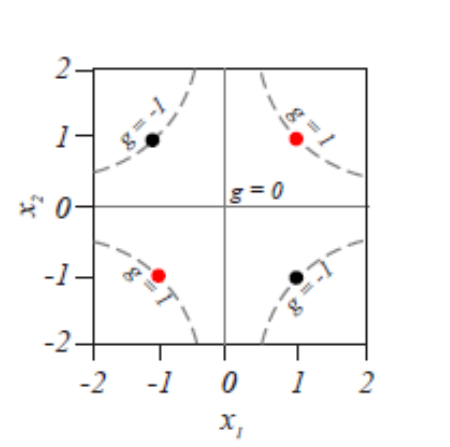
\includegraphics[width=0.4\textwidth]{exclusive_or.png}}}
		\caption{Exclusive-OR Problem}
		\label{exclusive_or}
	\end{figure}
		
	First, we transform the data using the $\varphi$ functions. The resulting data is given as follows:
	
	$\mathbf{x_1} = \varphi(\mathbf{x_1}) = [1,\sqrt{2},\sqrt{2},\sqrt{2},1,1]^T$
	
	$\mathbf{x_2} = \varphi(\mathbf{x_2}) = [1,\sqrt{2},-\sqrt{2},-\sqrt{2},1,1]^T$
	
	$\mathbf{x_3} = \varphi(\mathbf{x_3}) = [1,-\sqrt{2},-\sqrt{2},\sqrt{2},1,1]^T$
	
	$\mathbf{x_4} = \varphi(\mathbf{x_4}) = [1,-\sqrt{2},\sqrt{2},-\sqrt{2},1,1]^T$
	
	Next, we want to find $\alpha_1$, $\alpha_2$, $\alpha_3$, and $\alpha_4$ which maximize:
	
	$Q(\boldsymbol{\alpha}) = \sum{a_i} - \frac{1}{2}\sum{\sum{\alpha_i\alpha_jy_iy_j\mathbf{x_i}^T\mathbf{x_j}}}$.
	
	subject to $\sum{a_iy_i} = 0$ and $\alpha_i > 0\ \forall\ i$.
	
	Start by writing $Q(\boldsymbol{\alpha})$ in matrix form:

	Let $\mathbf{f} = [1,1,1,1]^T$ and $\boldsymbol{\alpha} = [\alpha_1, \alpha_2, \alpha_3, \alpha_4]^T$.
	
	Then, $\sum{a_i} = \mathbf{f}^T\boldsymbol{\alpha}$
	
	Next, define $\mathbf{\hat{x}_i} = y_i\mathbf{x_i}$, $\mathbf{\hat{X}} = [\mathbf{\hat{x}_1},\mathbf{\hat{x}_2}, \mathbf{\hat{x}_3}, \mathbf{\hat{x}_4}]$, and $\mathbf{H} = \mathbf{\hat{X}}^T\mathbf{\hat{X}}$
	
	Then, $\sum{\sum{\alpha_i\alpha_jy_iy_j\mathbf{x_i}^T\mathbf{x_j}}} = \boldsymbol{\alpha}^T\mathbf{H}\boldsymbol{\alpha}$ where $\mathbf{H}$ is symmetric.
	
	$\therefore Q(\boldsymbol{\alpha}) = \mathbf{f}^T\boldsymbol{\alpha} - \frac{1}{2}\boldsymbol{\alpha}^T\mathbf{H}\boldsymbol{\alpha}$
	
	Define $\mathbf{y} = [y_1, y_2, y_3, y_4]^T \Rightarrow \sum{\alpha_iy_i} = \mathbf{y}^T\boldsymbol{\alpha}$.
	
	$\therefore$ we are trying to maximize $Q(\boldsymbol{\alpha})$ subject to $\mathbf{y}^T\boldsymbol{\alpha} = 0$ and $\alpha_i > 0\ \forall\ i$
	
	Determine where $Q(\boldsymbol{\alpha})$ is maximized:
	
	$\nabla_{\boldsymbol{\alpha}}Q = \mathbf{f} - \mathbf{H}\boldsymbol{\alpha} = \mathbf{0} \Rightarrow \mathbf{H}\boldsymbol{\alpha} = \mathbf{f} \Rightarrow \boldsymbol{\alpha} = \mathbf{H}^{\dag}\mathbf{f} = \mathbf{H}^T(\mathbf{H}\mathbf{H}^T)^{-1}\mathbf{f}$
	
	Plugging in values for $\mathbf{H}$ and $\mathbf{f}$, we find $\boldsymbol{\alpha} = [1/8,1/8,1/8,1/8]^T$
	
	Note that $\mathbf{y} = [1, -1, 1, -1]^T \Rightarrow \mathbf{A}\boldsymbol{\alpha} = 0$. Further note that $\alpha_i > 0$.
	
	$\therefore$ we have found the value of $\boldsymbol{\alpha}$ which maximizes $Q(\boldsymbol{\alpha})$ subject to \newline $\mathbf{y}^T\boldsymbol{\alpha} = 0$ and $\alpha_i > 0$.
	
	For this case, note that the maximum of $Q(\boldsymbol{\alpha})$ just happened to satisfy the additional constraints. If this was not the case, it would be best to use linear programming to find the solution instead.
	
	Now, we can solve for $\mathbf{w}$ as follows:
	
	$\mathbf{w} = \sum{\alpha_iy_i\mathbf{x_i}} = \boldsymbol{\hat{X}}\boldsymbol{\alpha} = [0,0,0,1/\sqrt{2},0,0]^T$
	
	Finally, we can solve for $b$ as follows:
	
	$b = y_1 - \mathbf{w}^T\mathbf{x_1} = 1 - 1 = 0$
	
	The optimal discriminant $g(x_1,x_2)$ is then given as follows:
	
	$g(x_1,x_2) = \mathbf{w}^T\mathbf{x} + b = \frac{1}{\sqrt{2}}(\sqrt{2}x_1x_2) + 0 = x_1x_2$.
	
	\item Consider a Support Vector Machine and the following training data from two categories:
	
	\begin{center}
	\begin{tabular}{| c | c | c |}
		\hline
		category & $x_1$ & $x_2$ \\
		\hline
		$\omega_1$ & $1$ & $1$ \\
		$\omega_1$ & $2$ & $2$ \\
		$\omega_1$ & $2$ & $0$ \\
		\hline
		$\omega_2$ & $0$ & $0$ \\
		$\omega_2$ & $1$ & $0$ \\
		$\omega_2$ & $0$ & $1$ \\
		\hline
	\end{tabular}
	\end{center}
	
	\begin{enumerate}
		\item[(a)] Plot these six training points, and construct by inspection the weight vector for the optimal hyperplane, and the optimal margin.
		
		\begin{figure}[H]
			\centerline{\fbox{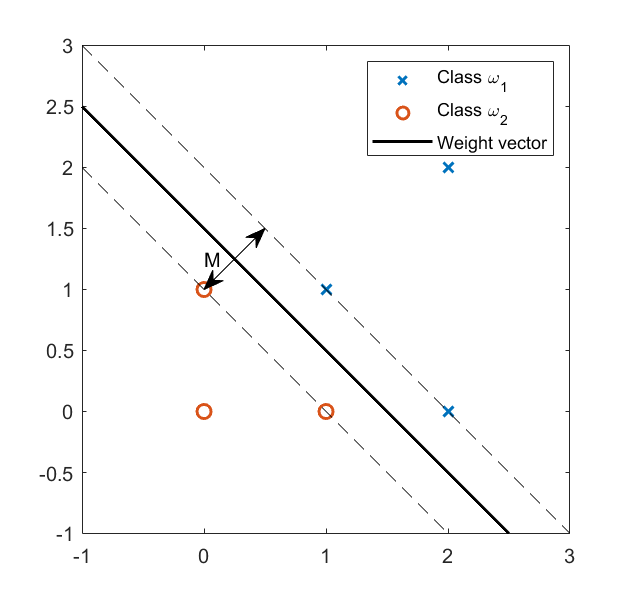
\includegraphics[width=0.8\textwidth]{solution_by_inspection.png}}}
			\caption{Training Samples with Weight Vector Found by Inspection}
			\label{solution_by_inspection}
		\end{figure}
		
		The linear discriminant function is given by inspection as:
		
		$y = -x + 1.5$		
		
		The weight vector is then given by scalar multiples of the following variables:
		
		\begin{equation*}
			\mathbf{w} = \begin{bmatrix} 1 \\ 1 \end{bmatrix} \text{ and } b = -1.5
		\end{equation*}
		
		We need to solve for the margin to determine the correct scaling.
		
		The optimal margin is given by
		
		\begin{equation*}
			M = 2\frac{\langle\mathbf{u}, \mathbf{v}\rangle}{\norm{\mathbf{v}}^2}
		\end{equation*}
		
		where $\mathbf{v} = \begin{bmatrix} 1 \\ -1 \end{bmatrix}$ and $\mathbf{u} = \begin{bmatrix} 0 \\ -0.5 \end{bmatrix}$
		
		\begin{equation*}
			\Rightarrow M = 2(0.5)/\sqrt{2} = 1/\sqrt{2} 
		\end{equation*}
		
		We can now solve for the required norm of the weight vector:
		
		\begin{equation*}
			M = \frac{2}{\norm{\mathbf{w}}} \Rightarrow \norm{\mathbf{w}} = \frac{2}{M} = 2\sqrt{2}
		\end{equation*}
		
		$\mathbf{w}$ currently has a norm of $\sqrt{2}$, so we must scale $\mathbf{w}$ and $b$ by $2$. Doing so results in the following:
		
		\begin{equation*}
			\mathbf{w} = \begin{bmatrix} 2 \\ 2 \end{bmatrix} \text{ and } b = -3
		\end{equation*}	
		
		\item[(b)] What are the support vectors?
		
		The support vectors are the datapoints which the margin pushes up against. Referring to Figure \ref{solution_by_inspection}, the support vectors are given by:
		
		$\mathbf{x} = [0, 1]^T$, $\mathbf{x} = [1, 0]^T$, $\mathbf{x} = [1, 1]^T$, and $\mathbf{x} = [2, 0]^T$
		
		\item[(c)] Construct the solution in the dual space by finding the Lagrange undetermined multipliers, $\alpha_i$. Compare your result to that in \newline part (a).
		
		To find the support vectors, and the corresponding weight vector, we need to maximize		
		
		$Q(\boldsymbol{\alpha}) = \sum{a_i} - \frac{1}{2}\sum{\sum{\alpha_i\alpha_jy_iy_j\mathbf{x_i}^T\mathbf{x_j}}}$.
	
	subject to $\sum{a_iy_i} = 0$ and $\alpha_i > 0\ \forall\ i$.
	
		As demonstrated in problem 1, we can rewrite these equations in matrix-vector form. This results in us maximizing
		
		$Q(\boldsymbol{\alpha}) = \mathbf{f}^T\boldsymbol{\alpha} - \frac{1}{2}\boldsymbol{\alpha}^T\mathbf{H}\boldsymbol{\alpha}$
		
		subject to $\mathbf{y}^T\boldsymbol{\alpha} = 0$ and $\alpha_i > 0\ \forall\ i > 0$.
		
		In the above equations, $\mathbf{f} = [1, ..., 1]^T$, $\boldsymbol{\alpha} = [\alpha_1, ..., \alpha_N]^T$, \newline $\mathbf{y} = [y_1,...,y_N]^T$, and $\mathbf{H} = \mathbf{\hat{X}}^T\mathbf{\hat{X}}$ with $\mathbf{\hat{X}} = [\mathbf{\hat{x}_1}, ..., \mathbf{\hat{x}_N}]^T$ \newline and $\mathbf{\hat{x}_i} = y_i\mathbf{x_i}$.

		We can use constrained optimization, to determine $\boldsymbol{\alpha}$, which \newline maximizes $Q(\boldsymbol{\alpha})$ subject to $\mathbf{y}^T\boldsymbol{\alpha} = 0$.
		
		Define the Lagrangian as $L(\boldsymbol{\alpha},\lambda) = Q(\boldsymbol{\alpha}) + \lambda g(\boldsymbol{\alpha})$ where $g(\boldsymbol{\alpha}) = \mathbf{y}^T\boldsymbol{\alpha}$
		
		$\Rightarrow L(\boldsymbol{\alpha},\lambda) = \mathbf{f}^T\boldsymbol{\alpha} - \frac{1}{2}\boldsymbol{\alpha}^T\mathbf{H}\boldsymbol{\alpha} + \lambda(\mathbf{y}^T\boldsymbol{\alpha})$
		
		At the constrained maximum, $\nabla_{\boldsymbol{\alpha}}L(\boldsymbol{\alpha},\lambda) = 0$ and $\nabla_{\lambda}L(\boldsymbol{\alpha},\lambda) = 0$ 
		
		$\Rightarrow \nabla_{\boldsymbol{\alpha}}L(\boldsymbol{\alpha},\lambda) = \mathbf{f} - \mathbf{H}\boldsymbol{\alpha} + \lambda\mathbf{y} = \mathbf{0} \Rightarrow \mathbf{H}\boldsymbol{\alpha} - \lambda\mathbf{y} = \mathbf{f}$
		
		$\Rightarrow \nabla_{\lambda}L(\boldsymbol{\alpha},\lambda) = \mathbf{y}^T\boldsymbol{\alpha} = \mathbf{0}$
		
		Let $\mathbf{x} = \begin{bmatrix} \boldsymbol{\alpha}\\ \lambda \end{bmatrix}$, $\mathbf{A} = \begin{bmatrix} \mathbf{H} & -\mathbf{y}\\ \mathbf{y}^T & 0 \end{bmatrix}$ and $\mathbf{b} = \begin{bmatrix} \mathbf{f} \\ 0\end{bmatrix}$
		
		Then, the set of equations can be rewritten as follows:
		
		$\mathbf{A}\mathbf{x} = \mathbf{b}$
		
		The above equation does not enforce $\alpha_i \geq 0$.
		
		Therefore, we have to force $\alpha_i = 0$ for all combinations of $\alpha_i$ and observe the result.
		
		To force a given $\alpha_i = 0$, we should zero out to column in $\mathbf{A}$ which corresponds to that $\alpha_i$. Additionally, we should remove the row in the matrix-vector equation which corresponds to $\frac{\partial{L(\boldsymbol{\alpha},\lambda)}}{\partial\alpha_i} = 0$
		
		 If the resulting equation does not have a valid solution or results in any $\alpha_i < 0$, the set of non-zero $\alpha_i$'s is incorrect.
		 
		 To determine the best selection of $\alpha_i$, we can compare $Q(\boldsymbol{\alpha})$ for all valid combinations of $\alpha_i$. The collection of $\alpha_i$ which maximizes $Q(\boldsymbol{\alpha})$ is the solution.
		
		To save time, we can use knowledge of the support vectors from part (b) to determine which $\alpha_i$ to set to zero. This results in the following matrix-vector equation:
		
		\begin{equation*}
			\begin{bmatrix}
				 2 & 0 &  2 & 0 & -1 & -1 & -1 \\
             	 2 & 0 &  4 & 0 & -2 &  0 & -1 \\
            		-1 & 0 & -2 & 0 &  1 &  0 &  1 \\
               	-1 & 0 &  0 & 0 &  0 &  1 &  1 \\
                	 1 & 0 &  1 & 0 & -1 & -1 &  0
			\end{bmatrix}\begin{bmatrix}
				\boldsymbol{\alpha} \\ \lambda
			\end{bmatrix} = \begin{bmatrix}
				1 \\ 1 \\ 1 \\ 1 \\ 0
			\end{bmatrix}
		\end{equation*}
		
		We can now convert this matrix to reduced row echelon form:
		
		\begin{equation*}
			\begin{bmatrix}[ccccccc|c]
				 2 & 0 &  2 & 0 & -1 & -1 & -1 & 1\\
             	 2 & 0 &  4 & 0 & -2 &  0 & -1 & 1\\
            		-1 & 0 & -2 & 0 &  1 &  0 &  1 & 1\\
               	-1 & 0 &  0 & 0 &  0 &  1 &  1 & 1\\
                	 1 & 0 &  1 & 0 & -1 & -1 &  0 & 0
			\end{bmatrix}
		\end{equation*}
		
		\begin{equation*}
			\Rightarrow \begin{bmatrix}[ccccccc|c]
				1 & 0 & 0 & 0 & 0 & -1 & 0 & 2 \\
     			0 & 0 & 1 & 0 & 0 &  1 & 0 & 2 \\
               	0 & 0 & 0 & 0 & 1 &  1 & 0 & 4 \\
     			0 & 0 & 0 & 0 & 0 &  0 & 1 & 3 \\
     			0 & 0 & 0 & 0 & 0 &  0 & 0 & 0
			\end{bmatrix}
		\end{equation*}
		
		The resulting matrix corresponds to the following set of equations:
		
		\begin{equation*}
			\begin{cases}
				\alpha_1 - \alpha_6 = 2 \\
				\alpha_3 + \alpha_6 = 2 \\
				\alpha_5 + \alpha_6 = 4
			\end{cases} \Rightarrow \begin{cases}
				\alpha_1 = 2 + \alpha_6 \\
				\alpha_3 = 2 - \alpha_6 \\
				\alpha_5 = 4 - \alpha_6
			\end{cases}
		\end{equation*}
		
		For a valid solution to exist, $\alpha_i \geq 0\ \forall\ i$. In this case, we see that the condition is met for $0 \leq \alpha_6 \leq 2$. Choose $\alpha_6 = 1$
		
		$\Rightarrow \alpha_1 = 3, \alpha_3 = 1, \alpha_5 = 3$
		
		$\Rightarrow\boldsymbol{\alpha} = [3,0,1,0,3,1]^T$
		
		Next, we can solve for $\mathbf{w}$ as follows:
		
		$\mathbf{w} = \sum{\alpha_iy_i\mathbf{x_i}} = \mathbf{\hat{X}}\boldsymbol{\alpha} = \begin{bmatrix} 2 \\ 2 \end{bmatrix}$
		
		Then, we can solve for $b$ as follows:
	
		$b = y_1 - \mathbf{w}^T\mathbf{x_1} = 1 - (2(1) + 2(1)) = 1 - 4 = -3$
		
		Finally, we can solve for the margin as follows:
		
		\begin{equation*}
			M = \frac{2}{\norm{\mathbf{w}}} = \frac{2}{\sqrt{2^2 + 2^2}} = \frac{2}{\sqrt{8}} = \frac{2}{2\sqrt{2}} = \frac{1}{\sqrt{2}}
		\end{equation*}
		
		This matches the result from part (a).
		
	\end{enumerate}
	
	\item The linear programming problem discussed in class involved minimizing a single artificial variable $\tau$ under the constraints $\mathbf{a}^T\mathbf{y_i} + \tau > b_i$ and $\tau \geq 0$. Show that the resulting weight vector minimizes the criterion function
	
	\begin{equation*}
		J_{\tau}(\mathbf{a}) = \underset{\mathbf{a}^T\mathbf{y_i} \leq b_i}{\text{max}}[b_i - \mathbf{a}^T\mathbf{y_i}]
	\end{equation*}
	
	Here, $\mathbf{a}$ is the weight vectors, $\mathbf{y_i}$ are the data vectors, and $b_i$ are the scalar constants.
	
	$\mathbf{a}^T\mathbf{y_i} + \tau > b_i \Rightarrow \tau > b_i -  \mathbf{a}^T\mathbf{y_i}$
	
	Because we are trying to minimize $\tau$ with $\tau \geq 0$, the final value of $\tau$ corresponds to $\underset{\mathbf{a}^T\mathbf{y_i} \leq b_i}{\text{max}}[b_i - \mathbf{a}^T\mathbf{y_i}]$.
	
	$\therefore$ by minimizing $\tau$, we are also minimizing the criterion function $J_{\tau}(\mathbf{a})$
	
	\end{enumerate}
\end{document}